\section{mo\-Rand\-Move$<$ M $>$ Class Template Reference}
\label{classmo_rand_move}\index{moRandMove@{moRandMove}}
Random move generator.  


{\tt \#include $<$mo\-Rand\-Move.h$>$}

Inheritance diagram for mo\-Rand\-Move$<$ M $>$::\begin{figure}[H]
\begin{center}
\leavevmode
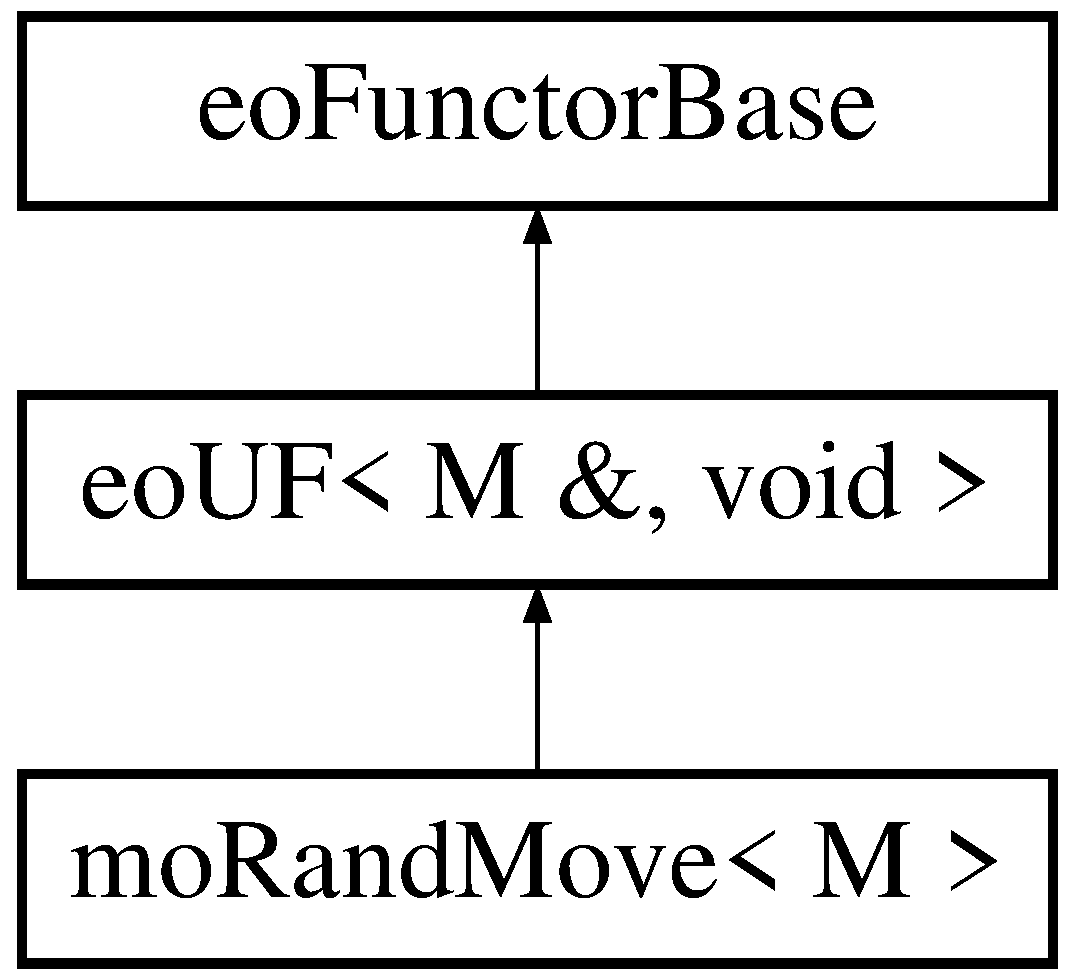
\includegraphics[height=3cm]{classmo_rand_move}
\end{center}
\end{figure}


\subsection{Detailed Description}
\subsubsection*{template$<$class M$>$ class mo\-Rand\-Move$<$ M $>$}

Random move generator. 

Only a description... An object that herits from this class needs to be designed in order to use a {\bf mo\-SA}{\rm (p.\,\pageref{classmo_s_a})}. 



Definition at line 46 of file mo\-Rand\-Move.h.

The documentation for this class was generated from the following file:\begin{CompactItemize}
\item 
mo\-Rand\-Move.h\end{CompactItemize}
